\documentclass[master.tex]{subfiles}
\begin{document}

\chapter{Example Formal System --- Simple Arithmetic}
\label{chap:example_simple_arithmetic}

As in \hyperref[chap:background]{background chapter}, Simple Arithmetic is
used as example to explain basic concept of formal systems and its derivations.
In order to make the transition goes smoother, this chapter aims to encode
Simple Arithmetic and explain basic features and usability of \emph{Phometa} at
the same time. Please note that this is just a faction of
actual arithmetic modified to make it easier to understand, so it is not as
powerful as the actual one.

\section{First time with Phometa}

You can download complied version of Phometa at

{\centering\url{https://github.com/gunpinyo/phometa/raw/master/build/phometa.tar.gz}}

Once you unzip this file, you can start Phometa server by execute

\texttt{./phometa-server.py 8080}

where \texttt{8080} is port number, you can change this to another port number
if you like. Please note that Python is required for this server.

Then open your favourite web-browser\footnote{but Google Chrome is recommended}
and enter

\texttt{http://localhost:8080/phometa.html}

The program will look like this

\begin{figure}[H]
    \centering
    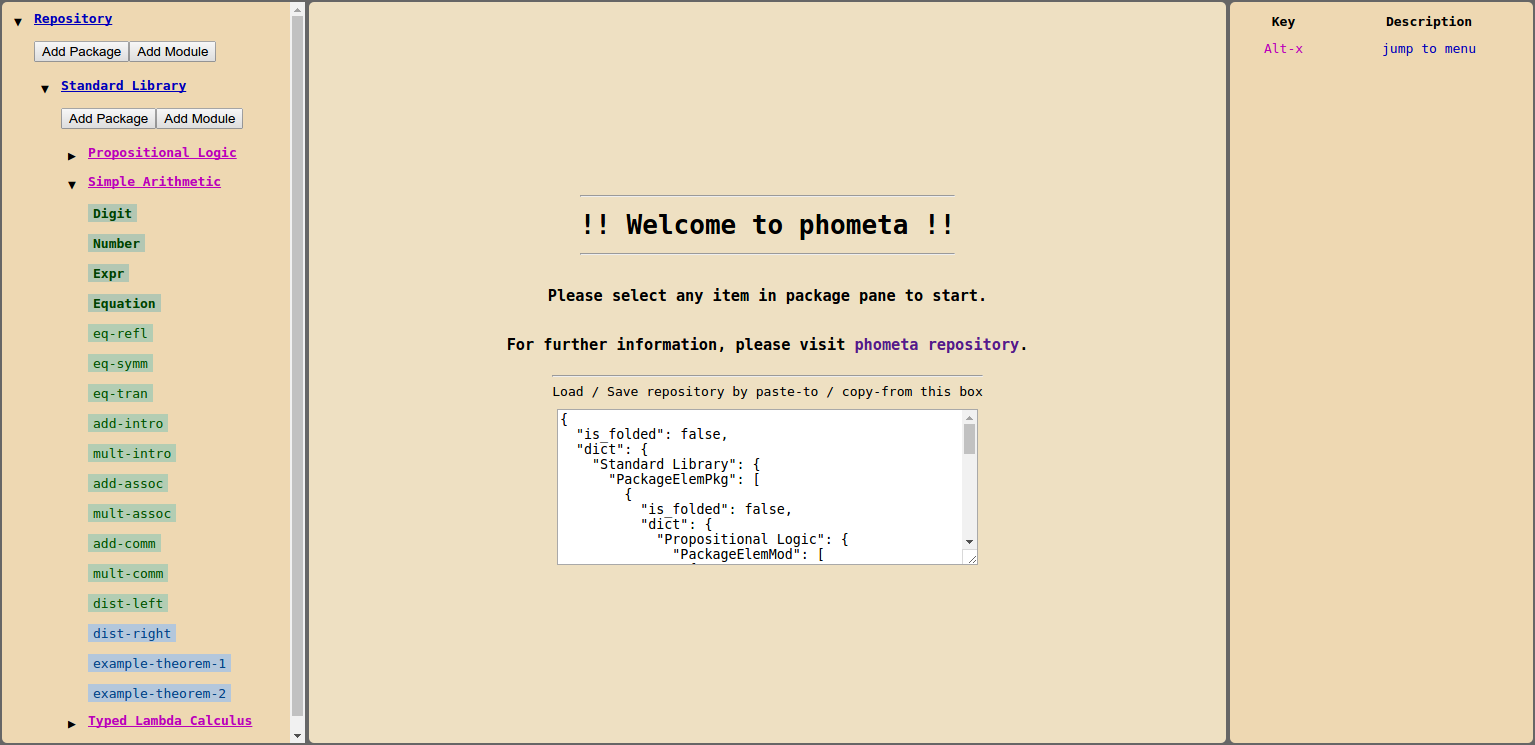
\includegraphics[width=\textwidth]{arith-phometa-home-window}
    \caption{Screenshot of Phometa when you open it from web-browser.}
\label{fig:arith-phometa-home-window}
\end{figure}

Phometa has a repository which consists of packages and modules that store
formal systems and its proofs. The left pane of figure
\ref{fig:arith-phometa-home-window} shows global structure of a repository. The
current repository has one package named ``Standard Library'' which consists of
three modules named ``Propositional Logic'', ``Simple Arithmetic'', and ``Typed
Lambda Calculus''.

Module in Phometa are analogous to text file. It consists of nodes that could
depend on one another. There are four types of node which are \emph{Comment},
\emph{Grammar} (Backus-Naur Form), \emph{Rule} (Derivation Rule), and
\emph{Theorem} (Derivation Tree). If you click at a module on the repository
pane e.g. ``Simple Arithmetic'', you will see the whole content of the module
appear on the centre pane. Alternatively, you can click on each node on the
repository pane directly to focus on particular node.

\begin{figure}[H]
    \centering
    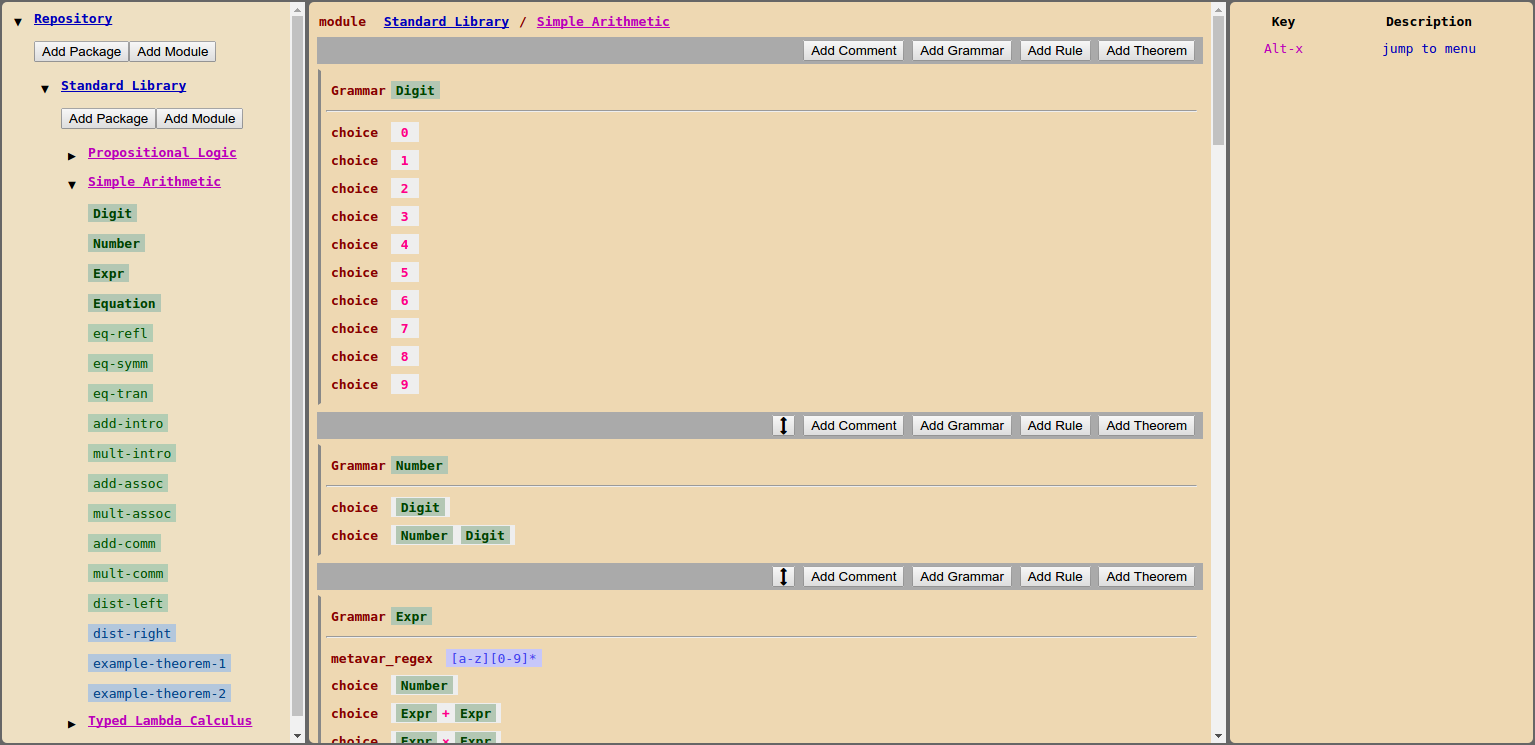
\includegraphics[width=\textwidth]{arith-phometa-arith-window}
    \caption{Screenshot of Phometa when you click ``Simple Arithmetic'' module.}
\label{fig:arith-phometa-arith-window}
\end{figure}

In order to improve productivity, Phometa has several key-bindings specific to
certain state of program. Fortunately, user don't need to remember any of this
since the right pane (i.e. keymap pane) shows every possible key-binding with
its description on current state. This also allow new-comer to explore new
features during using it

\section{Grammars}

The Backus-Naur Form of Simple Arithmetic in figure \ref{fig:background-bnf}
could be transformed in to this four following grammars
\begin{figure}[H]
    \centering
\begin{minipage}{0.7\textwidth}
    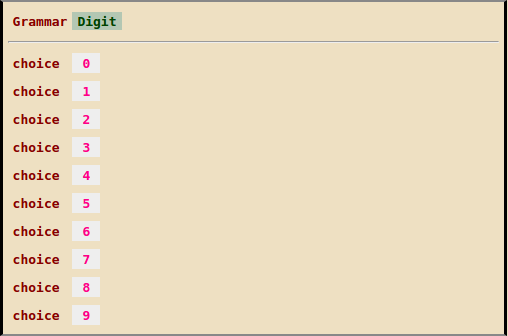
\includegraphics[width=\textwidth]{arith-grammar-digit}
    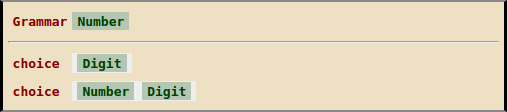
\includegraphics[width=\textwidth]{arith-grammar-number}
    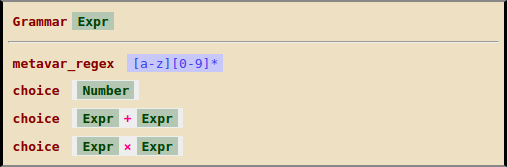
\includegraphics[width=\textwidth]{arith-grammar-expr}
    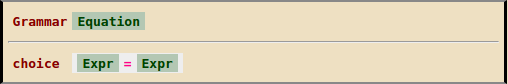
\includegraphics[width=\textwidth]{arith-grammar-equation}
\end{minipage}

    \caption{Grammars of Simple Arithmetic}
\label{fig:arith-grammars}
\end{figure}

We take advantage of visualisation by replacing brackets with underlines, this
should improve readability because reader can see a whole term in a compact
way but still able check how they are bounded when needed, for example,
\begin{itemize}
% \item \texttt{<Digit>} $2$ is transformed to \pgmr{Digit} \term{arith-term-digit}
\item \texttt{<Number>} $250$ is transformed to
  \pgmr{Number} \term{arith-term-number}
\item \texttt{<Expr>} $(12 + (0 \times 6))$ is transformed to
  \pgmr{Expr} \term{arith-term-expr}
\item \texttt{<Equation>} $(5 + 7) = 12$ is transformed to
  \pgmr{Equation} \term{arith-term-equation}
\end{itemize}
These underline patterns coincide with diagram in figures \ref{fig:background-digit},
\ref{fig:background-number}, \ref{fig:background-expr-2}, and
\ref{fig:background-equation} respectively.

\kMetaVarRegex\ is used to control the name meta variables of each grammar. If
this property is omitted, the corresponding grammar cannot instantiate meta
variables. For example, \pgmr{Expr} can instantiate meta variables with the name
comply to regular expression \pregex{\texttt{[a-z][0-9]*}} (e.g. \pvar{a}, \pvar{b},
$\ldots$, \pvar{z}, \pvar{a1}, \pvar{a2}, $\ldots$), whereas \pgmr{Digit},
\pgmr{Number}, and \pgmr{Equation} couldn't instantiate any meta variables,
however, it could have meta variables as sub-term e.g. \pgmr{Equation}
\term{arith-term-equation-var}.

\section{Rules}

The derivation rules of Simple Arithmetic in figure \ref{fig:background-derivation-rules}
can be transformed as the following

\begin{center}
\begin{minipage}{0.6\textwidth}
    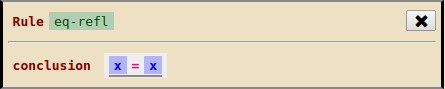
\includegraphics[width=\textwidth]{arith-rule-eq-refl}
    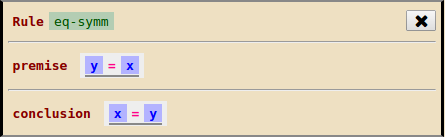
\includegraphics[width=\textwidth]{arith-rule-eq-symm}
    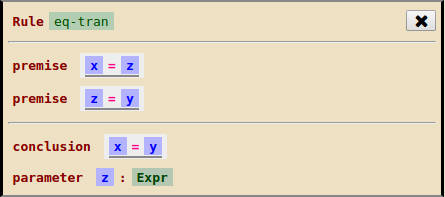
\includegraphics[width=\textwidth]{arith-rule-eq-tran}
\end{minipage}
\end{center}

\begin{figure}[H]
    \centering
\begin{minipage}{0.6\textwidth}
    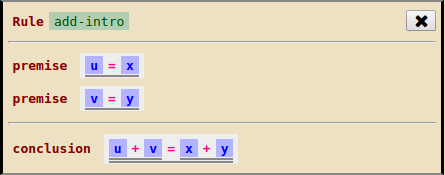
\includegraphics[width=\textwidth]{arith-rule-add-intro}
    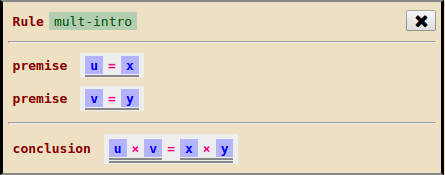
\includegraphics[width=\textwidth]{arith-rule-mult-intro}
    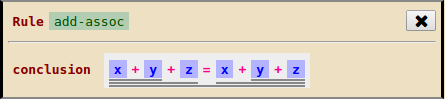
\includegraphics[width=\textwidth]{arith-rule-add-assoc}
    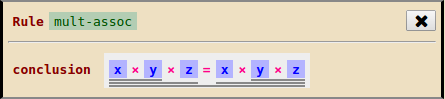
\includegraphics[width=\textwidth]{arith-rule-mult-assoc}
    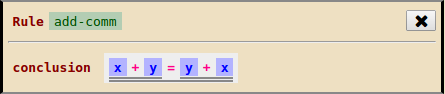
\includegraphics[width=\textwidth]{arith-rule-add-comm}
    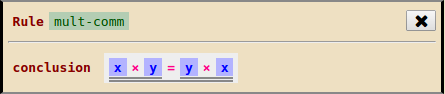
\includegraphics[width=\textwidth]{arith-rule-mult-comm}
    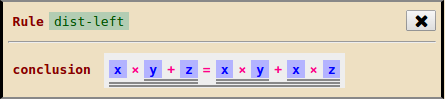
\includegraphics[width=\textwidth]{arith-rule-dist-left}
\end{minipage}
    \caption{Rules of Simple Arithmetic}
\label{fig:arith-rules}
\end{figure}

Most of rules here are self explain but in rule \prule{eq-tran}, there is an
additional property named \kParameter{}(s) which is a meta veritable that appear
in premises but not in conclusion, hence user need to give a term when the rule
is applied. Please note that \kParameter{} is automatic i.e.\ when user define
they own rule, it will change automatically depending on premises and conclusion

\pthm{dist-right} is not defined here but it will be defined as \emph{lemma}
in the next section.

\section{Theorems and Lemmas}

The first example of derivation tree (figure
\ref{fig:background-derivation-tree-1}) could be transformed to theorem

\begin{figure}[H]
    \centering
\begin{minipage}{0.8\textwidth}
    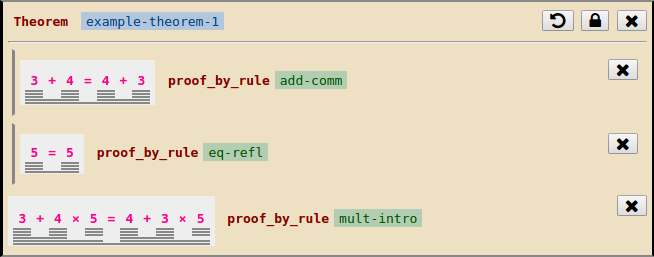
\includegraphics[width=\textwidth]{arith-theorem-example-theorem-1}
\end{minipage}
\caption{A theorem that show that $(3 + 4) \times 5 = (4 + 3) \times 5$.}
\label{fig:arith-theorem-example-theorem-1}
\end{figure}

You can see that the theorem still preserve tree-like structure but the width
doesn't grow exponentially like derivation.

Next, I will show you that how was the theorem above constructed. Once we click
module ``Simple Arithmetic'' on the repository pane, we will see the whole
context similar to figure \ref{fig:arith-phometa-arith-window}, you will also
see that there are adding panel intersperse among each node


\includegraphics[width=\textwidth]{arith-thm-ex-1}

Now, click ``Add Theorem'', the button will change to input box where you can
specify theorem name. Type ``tutorial-theorem-1'', can you will get empty
theorem as the following

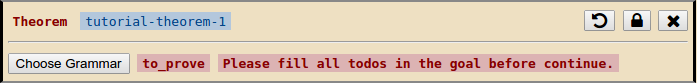
\includegraphics[width=\textwidth]{arith-thm-ex-2}

The first thing that we can do is to construct the goal that will be proven. On
the picture above you will see button labelled ``Choose Grammar'' which is, in
fact, a term that doesn't know its grammar. We can specify grammar by click the
button, which in-tern, will change to input box. Now the keymap pane will look
like this

\begin{center}
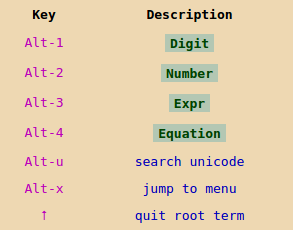
\includegraphics[width=0.4\textwidth]{arith-thm-ex-3}
\end{center}

The keymap pane told us that there are 4 grammars available, we can either press
\pkbd{Alt-{1..4}} or click on the row in keymap pane directly to select grammar.
Alternatively, you can search a grammars by type faction on it is input box e.g.
``eq''

\begin{center}
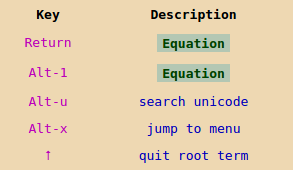
\includegraphics[width=0.4\textwidth]{arith-thm-ex-4}
\end{center}

Now, it is only \pgmr{Equation} available because it is the only one that has
``eq'' as (case-insensitively) sub-string. And since it is the only one, you can
select it by press \pkbd{Return}, even though in this case we don't have too
many options but still benefit from it in auto complete favour. Please note that
this input box support multiple matching separated by space e.g. ``eq ti'' still
match \pgmr{Equation} because both of ``eq'' and ``ti'' are sub-string of it.

Once you select a grammar, the box will change to green colour and waiting for a
term of that grammar. In this case, we select \pgmr{Equation} since it has just
one choice and doesn't have meta variable or literal\footnote{literal is similar
  to meta-variable but only match to itself, will be explained in later
  chapter} so Phometa automatically click such a choice and the theorem will
look like this

\begin{center}
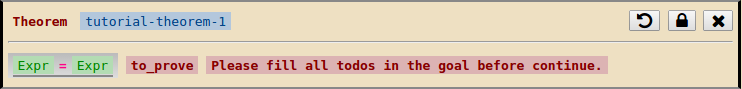
\includegraphics[width=\textwidth]{arith-thm-ex-5}
\end{center}

You may notice that the goal term as grey background rather than white as
before. This indicate that the term is still modifiable.

Next, we will continue on the \pgmr{Expr} term on the left hand side of
``$=$''. When the cursor is in it, the keymap will look like this

\begin{center}
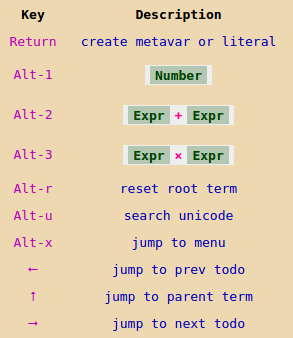
\includegraphics[width=0.4\textwidth]{arith-thm-ex-6}
\end{center}

Again, there are 3 choice available which can be selected similar manner when we
select grammar. At the this stage you might wonder how to type ``$\times$''
since it is unicode character. Well, we can go to unicode mode by press
\pkbd{Alt-u} as keymap pane suggest. Then keymap pane will look like this

\begin{center}
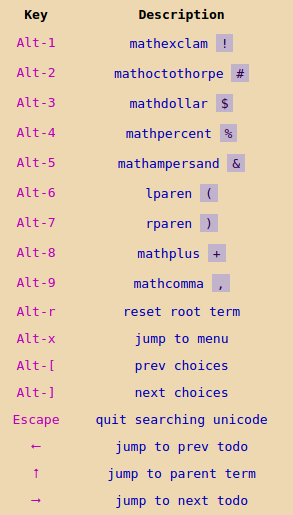
\includegraphics[width=0.3\textwidth]{arith-thm-ex-7}
\end{center}

This allow us to search unicode character by using its \LaTeX{}'s math-mode
name. Now type ``times'' in the input box, you should see ``$\times$'' appear on
keymap. Once you select it, the unicode mode disappear and put ``$\times$'' in
the input box, which in-tern, filter other choices out so you can hit
\pkbd{Return} for multiplication. The goal will transform to

\begin{center}

\includegraphics[width=0.2\textwidth]{arith-thm-ex-8}
\end{center}

\hspace{1ex}

Next we will focus middle \pgmr{Expr}. If we type string and hit \pkbd{Return}
here it will assume that we enter meta variable or literal (to avoid conflict
auto complete similar to choose grammar is disabled here). E.g.\ if we type ``a''
and press enter it will become like this

\begin{center}

\includegraphics[width=0.2\textwidth]{arith-thm-ex-9}
\end{center}

If we enter the name that that doesn't comply to regular expression, it will
do nothing and prompt error message above main pane as the following

\begin{center}

\includegraphics[width=\textwidth]{arith-thm-ex-10}
\end{center}

By the way, the goal here doesn't involve any meta variable. We can reset any
sub-term (e.g. in this case \pvar{a}) by pressing \pkbd{Alt-t}. Ultimately,
you can reset the whole term by pressing \pkbd{Alt-r}. In addition, you can jump
to parent term by pressing \pkbd{UP}, this is particularly useful when
combine with \pkbd{Alt-t} i.e.\ you can reset parent term only by keystrokes
rather than clicking. You also be able to jump to previous todo or next todo by
pressing \pkbd{LEFT} or \pkbd{RIGHT} respectively.

By recursively fill the the goal, eventually it will become like this

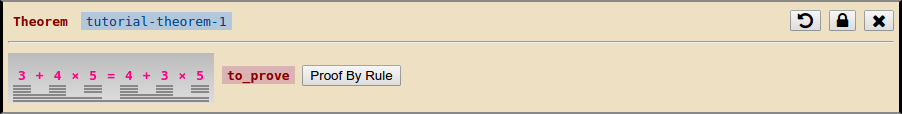
\includegraphics[width=\textwidth]{arith-thm-ex-11}

Since the goal is complete, it is ready to be proven. You can select a rule by
clicking ``Proof By Rule'' and select \prule{mult-intro} similar manner to
choose grammar. Then the theorem will look like this

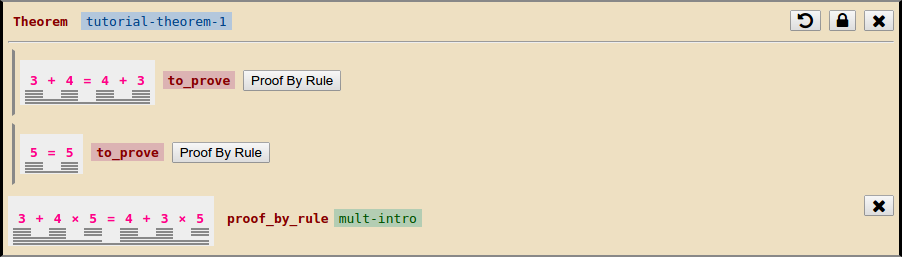
\includegraphics[width=\textwidth]{arith-thm-ex-12}

\hspace{1ex}

Once the rule is applied, it will generate further sub-goals.

Please notice that the goal background changes to white colour as we can longer
modify the goal. However if you made a mistake and want to go back, you can
click close button on the bottom right corner of current proof (or press
\pkbd{Alt-t}) to reset current proof then you can modify it again. Ultimately,
you can click reset button on the top right corner of the theorem (or press
\pkbd{Alt-r}) to reset entire theorem.

Two remaining sub-goals that have been generated can be proven similar to the
process above i.e.\ select rule \prule{add-comm} for first sub goal and
\prule{eq-refl} for second one.

\begin{center}
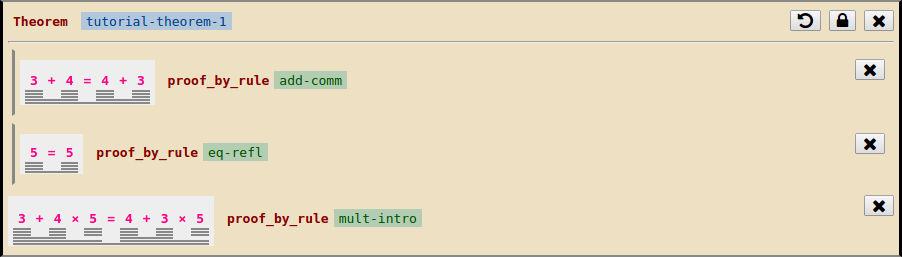
\includegraphics[width=\textwidth]{arith-thm-ex-13}
\end{center}

Once the theorem is complete, you can claim validity of the goal. More over you
can convert it to lemma that can be used in later theorem by clicking lock
button on top-right corner of theorem

\begin{center}
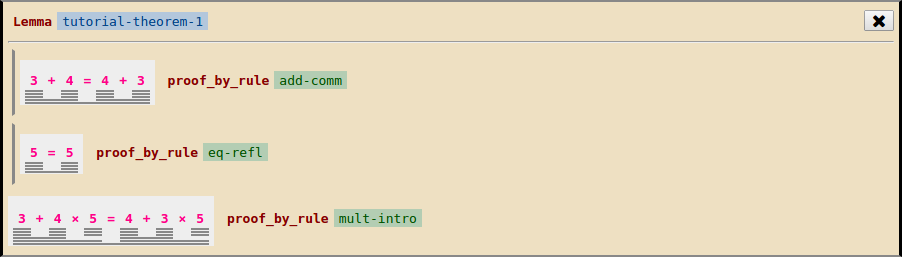
\includegraphics[width=\textwidth]{arith-thm-ex-14}
\end{center}

Because other theorem can use this lemma so it is no longer modifiable, as you
can see that close button of each sub-proof and reset button of the main theorem
are gone.

\newpage

Similarly, we can can create lemma \pthm{dist-right} as the following

\hspace{1ex}

\begin{figure}[H]
    \centering
\begin{minipage}{\textwidth}
    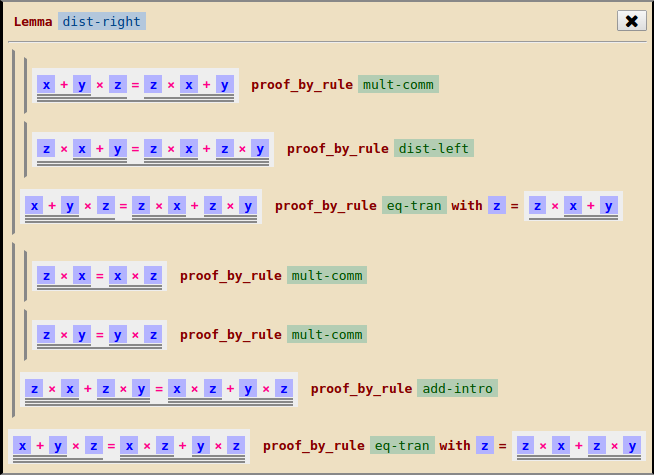
\includegraphics[width=\textwidth]{arith-lemma-dist-right}
\end{minipage}
\caption{An example of lemma obtained by lock a theorem.}
\label{fig:arith-lemma-dist-right}
\end{figure}

\hspace{1ex}

It is a good practice to create lots of small lemmas rather than a big theorem.
This is because it is easier to read and you can use a lemma multiple time i.e.
no need to duplicate sub-proof.


\section{More complex theorem}

To gain more familiarly on theorem, here is more complex theorem corresponded
the second example of derivation tree on figure \ref{fig:background-derivation-tree-2}

\begin{figure}[H]
    \centering
\begin{minipage}{\textwidth}
    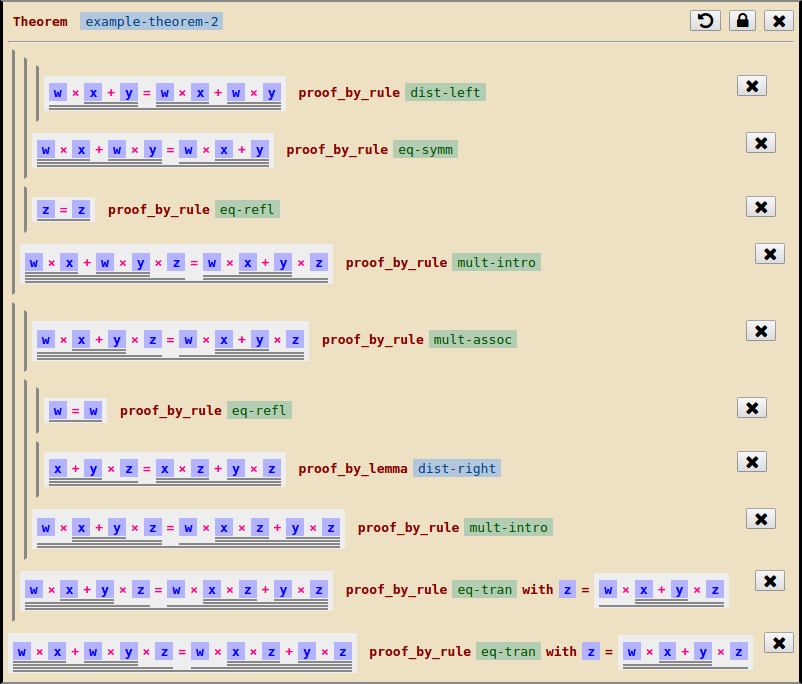
\includegraphics[width=\textwidth]{arith-theorem-example-theorem-2}
\end{minipage}
\caption{The second example theorem of Simple Arithmetic.}
\label{fig:arith-theorem-example-theorem-2}
\end{figure}

Sub-proofs become more complex and premises of main proof are far away which
is harder to read, to avoid this kind of problem, we introduce a focus button
that will fold sub-proof of corresponding proof. For example, if we click
focus button on the main proof it will look like this

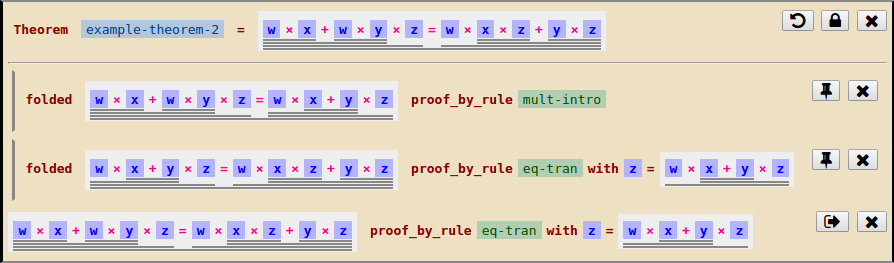
\includegraphics[width=\textwidth]{arith-thm-ex-focus-1}

Two sub-proofs of the main theorem are folded, this allow us to read rule
instance of \prule{eq-tran} easily. You can unfolded sub-proofs by clicking
unfocus button at the same position that focus button was there before. And the
theorem will look the same as figure \ref{fig:arith-theorem-example-theorem-2}
again.

When you read some proof in Phometa, it is a good idea to click focus on the
main proof first so you can read the main rule instance easily. Once you
understand main proof you can read one of sub proof by clicking focus button
that correspond to that sub-proof. If you click focus button on the first
sub-proof it will look like this

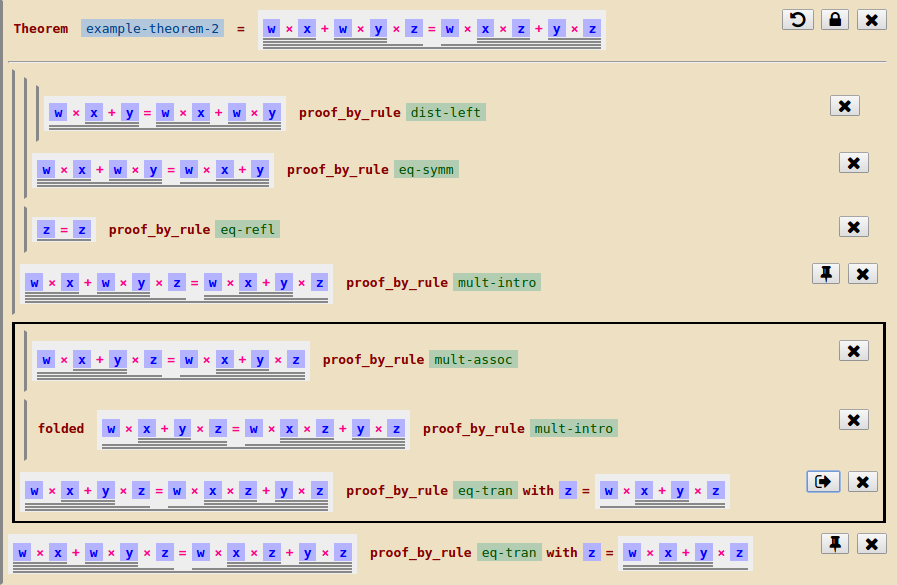
\includegraphics[width=\textwidth]{arith-thm-ex-focus-2}

This process automatically unfold the previous one before folding sub-proof
of this proof again. Please note that some of deeper proofs might not have
focus button at all, this is because its sub-proofs cannot reduce further than
original one.

The next thing that I will show are how to use rule parameters and lemma. This
can be illustrated by recreate this theorem again. First create create a theorem
\pthm{tutorial-theorem-2} using the same goal as above theorem.

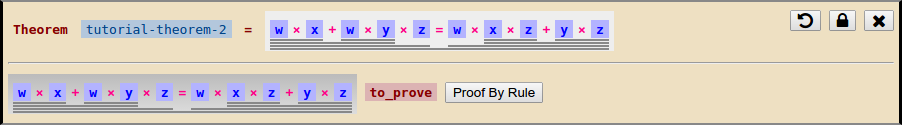
\includegraphics[width=\textwidth]{arith-thm-ex-15}

Then apply rule \prule{eq-tran} to this goal

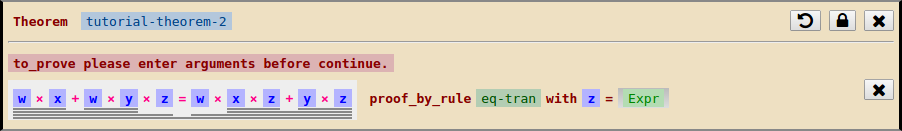
\includegraphics[width=\textwidth]{arith-thm-ex-16}

The rule applying process is not complete because \prule{eq-tran} contains
\pvar{z} which appear in premises but not in conclusion (i.e. \pvar{z} is
parameter) so Phometa ask us to fill the term that we want to use. In this case
we want \term{arith-thm-ex-aux-1} so put it there

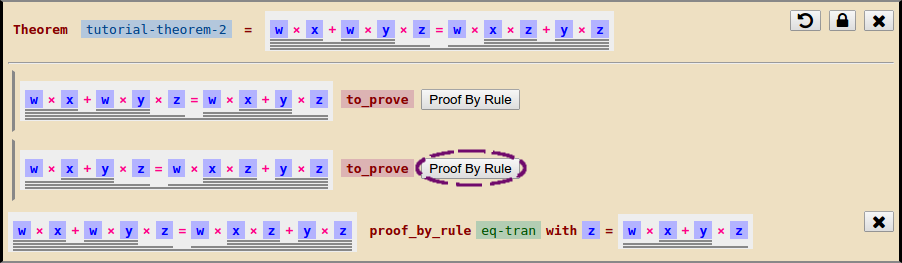
\includegraphics[width=\textwidth]{arith-thm-ex-17}

Now, let focus on the second sub-goal, we can apply \prule{eq-tran} again but
with \\ \pvar{z} = \term{arith-thm-ex-aux-2}. Then, apply \prule{mult-intro} in the second its sub-goal.

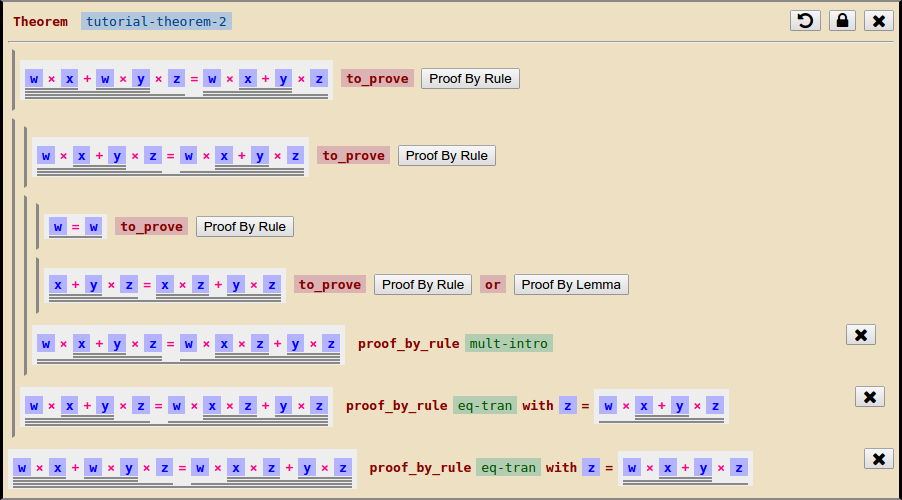
\includegraphics[width=\textwidth]{arith-thm-ex-18}

\hspace{1ex}

You can see that there is a sub-goal that has button ``Proof By Lemma''. This is
because there is at least one lemma that is pattern matchable with that
sub-goal. If you click ``Proof By Lemma'' button, the keymap will look like this

\begin{center}
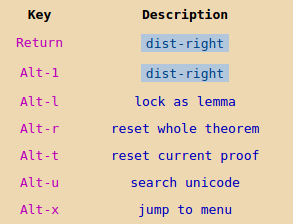
\includegraphics[width=0.4\textwidth]{arith-thm-ex-19}
\end{center}

In this case, there is one lemma which is \pthm{dist-right} that is pattern
matchable to that sub-goal. You can hit \pkbd{Return} to use this lemma and it
will look like this

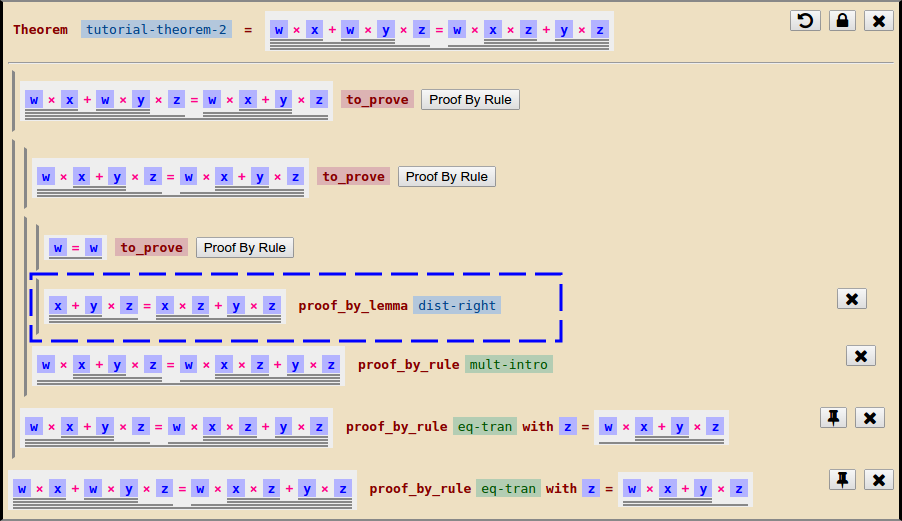
\includegraphics[width=\textwidth]{arith-thm-ex-20}

The remaining step is easy enough.

\newpage
\section{Exercises}

\begin{itemize}
\item Create a theorem and proof each of the following
  \begin{itemize}
  \item \term{arith-ex-1-1}
  \item \term{arith-ex-1-2}
  \item \term{arith-ex-1-3}
  \end{itemize}
\item Create a theorem of your own choice and proof it.
\item (Challenge) Extend Simple Arithmetic to support the following
  \begin{itemize}
  \item addition and multiplication identity.
  \item addition and multiplication idempotent.
  \item inequality.
  \end{itemize}
  You may need to create a new grammar or rules for this, please see section
  \ref{sec:how_to_built_grammars_and_rules} in the next chapter.
\end{itemize}
\end{document}